\section{Resultados}

A seção de "Resultados" em um relatório técnico-científico serve para apresentar os dados coletados durante o experimento ou pesquisa. Ela fornece evidências concretas para apoiar as conclusões tiradas na seção de "Metodologia" (para esse primeiro projeto, não será necessário o uso da metodologia), permitindo aos leitores avaliar a validade das conclusões apresentadas. Além disso, os resultados também são comparados com as expectativas iniciais e analisados quanto a padrões, tendências e relações entre os dados. Em resumo, os resultados são a base empírica para as conclusões do relatório. \\

\begin{figure}[h]
        \centering
        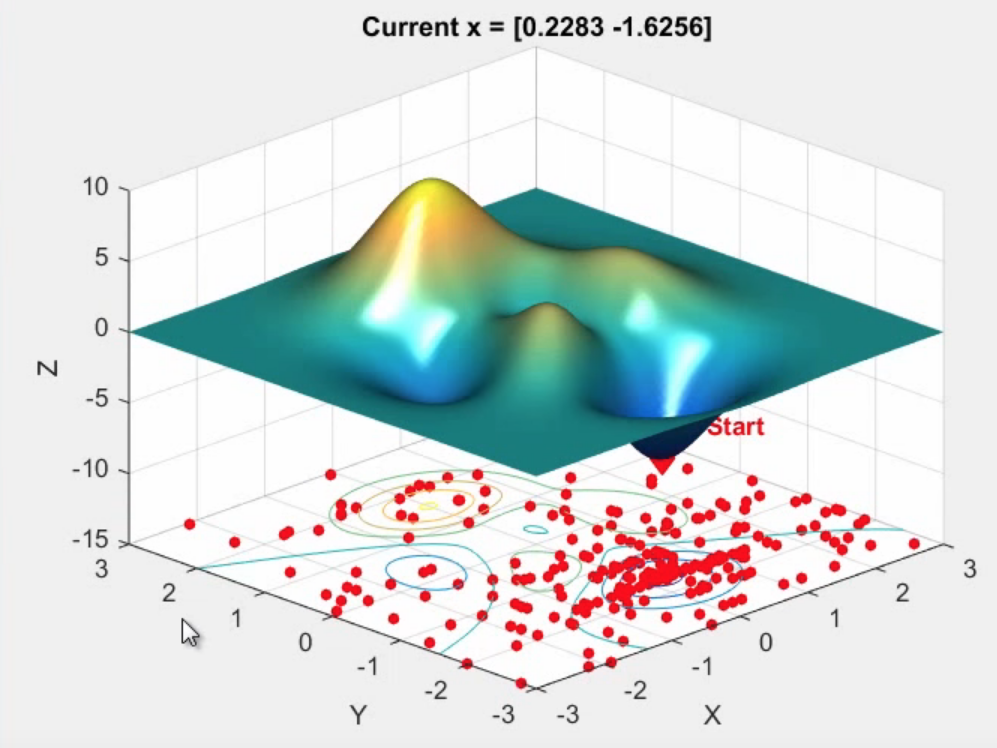
\includegraphics[width=0.75\textwidth]{images/final1.png}
    \caption{Laamarti, Eid e El Saddik, Acredite}
    \label{fig:test}
\end{figure}

Fusce mauris. Vestibulum luctus nibh at lectus. Sed bibendum, nulla a faucibus semper, leo
velit ultricies tellus, ac venenatis arcu wisi vel nisl. Vestibulum diam. Aliquam pellentesque,
augue quis sagittis posuere, turpis lacus congue quam, in hendrerit risus eros eget felis.
Maecenas eget erat in sapien mattis porttitor. Vestibulum porttitor. Nulla facilisi. Sed a
turpis eu lacus commodo facilisis. Morbi fringilla, wisi in dignissim interdum, justo lectus
sagittis dui, et vehicula libero dui cursus dui. Mauris tempor ligula sed lacus. Duis cursus
enim ut augue. Cras ac magna. Cras nulla. Nulla egestas. Curabitur a leo. Quisque egestas
wisi eget nunc. Nam feugiat lacus vel est. Curabitur consectetuer. \\
